\chapter{超导量子比特的控制与测量}
前面已经介绍了超导量子计算系统的基本结构和基本原理,我们现在已经获得了多比特耦合的超导量子处理器以及支持计算过程的信号产生与传输系统。但是想要进行完整的超导量子计算过程,我们还需要对信号控制量子比特状态的过程有清晰的认知。接下来,我们将从整个量子计算过程的角度,介绍超导量子比特在计算前的初态制备过程,计算过程中的状态操控过程,以及最终对超导量子比特的状态读取。
\section{超导量子比特的初态制备}
进行超导量子计算的第一步就是将超导量子比特的状态制备到量子算法所需要的初态。我们一般是从系统的$\ket{0}$态出发,通过一系列单比特门操作和双比特门操作将系统制备到所需初态,量子门操作将在下一部分进行详细介绍,本节将主要介绍如何将系统制备到$\ket{0}$态。将系统制备到$\ket{0}$态主要依靠系统的能量弛豫,系统与周围环境进行耦合,当系统的能量全部耗散到环境中,系统就自然处于$\ket{0}$态。根据在耗散过程中是否施加加速耗散的操作,我们可以将初态$\ket{0}$态制备分为主动重置和被动重置两种。
\subsection{被动重置}
被动重置就是在系统弛豫到$\ket{0}$态的过程中不施加任何操作。超导量子比特与周围环境进行耦合,不断有能量流失到周围环境中,当大部分能量耗散到环境中,量子比特储存的信息也相应的丢失了,因此量子比特都会有一个能量弛豫时间$T_{1}$,用以表征量子比特能量弛豫的快慢。一般在量子线路结束后,我们会将量子比特静置等待五倍的$T_{1}$时间,就可以系统绝大部分制备到0态,$\ket{1}$态的占据数小于$1\% $,接下来就可以开始下一轮的量子线路。一般而言,当前的$T_{1}$时间达到了百微秒量级,因此静置等待时间也要百微秒甚至毫秒量级,极大延缓了量子计算的速度。为了减少等待的时间,提高量子计算的速度,某些研究组研发了主动重置技术。

\subsection{主动重置}
主动重置和被动重置的过程类似,只是会在能量弛豫过程中对量子比特施加操控,加速能量弛豫的速度。目前的主动重置过程一般都是增强量子比特与读取腔的相互作用,因为读取腔与周围环境有极强的耦合,所以量子比特与环境的耦合也会显著增强,大大减少能量弛豫时间$T_{1}$,可以在百纳秒的时间内将系统的$\ket{1}$态弛豫到$1\% $。

具体的操控方式有两种,一种是施加方波或者MHz量级的微波,将量子比特频率靠近读取腔频率,如下图\ref{fig:reset1}b所示。利用这种方式增大比特与读取腔的等效耦合强度,能量从比特传输到读取腔,进而快速耗散到环境中,如下图\ref{fig:reset1}a所示。施加方波的重置方式在操作上更简单,速度上也相对较快,但是在硬件上有限制,需要读取腔频率低于比特频率。施加$MHz$量级微波的方式没有硬件频率的限制,但是操作上更复杂一点,而且等效耦合强度较低,重置的速度也比较慢。

\begin{figure}[h]
	\centering
	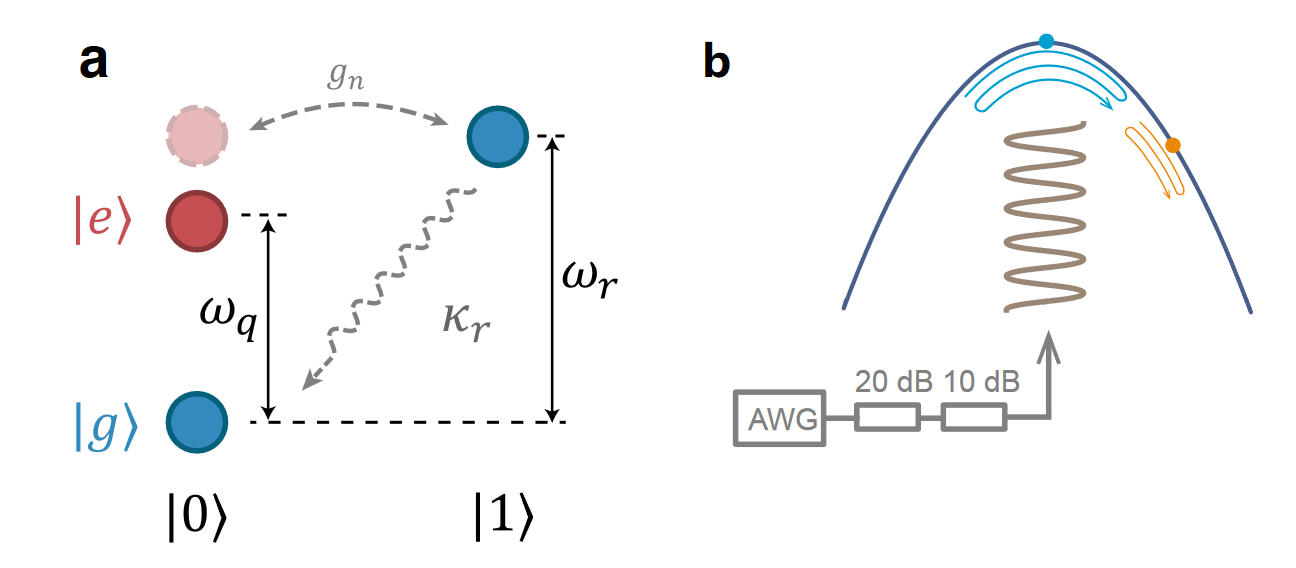
\includegraphics[width=0.7\textwidth]{reset1.png}
	\caption{施加MHz量级的微波实现比特状态重置示意图\cite{zhou2021rapid}。a)利用MHz量级的微波实现比特状态重置的物理过程,通过微波将比特频率与读取腔频率对齐,将能量从比特转移到读取腔中,实现能量的快速耗散。b)所施加的MHz量级微波波形示意图,实现比特频率的周期振荡。}
	\label{fig:reset1}
\end{figure}

另一种方式是施加GHz量级微波驱动,如图\ref{fig:reset2}所示,将系统的$\ket{10}$态,$\ket{20}$态和$\ket{01}$态通过微波驱动耦合起来,其中前一个数字代表比特状态,后一个数字代表读取腔状态,也就是将比特的$\ket{1}$态和$\ket{2}$态转移到读取腔的$\ket{1}$态。读取腔的$\ket{1}$态能量进而快速耗散到环境中,从而将整个量子比特系统弛豫到$\ket{0}$态。这种方案同样没有硬件频率的限制,重置速度也比$MHz$量级微波的方案更快,但是因为对比特有能量驱动,对操作精度的要求更高。

\begin{figure}[h]
	\centering
	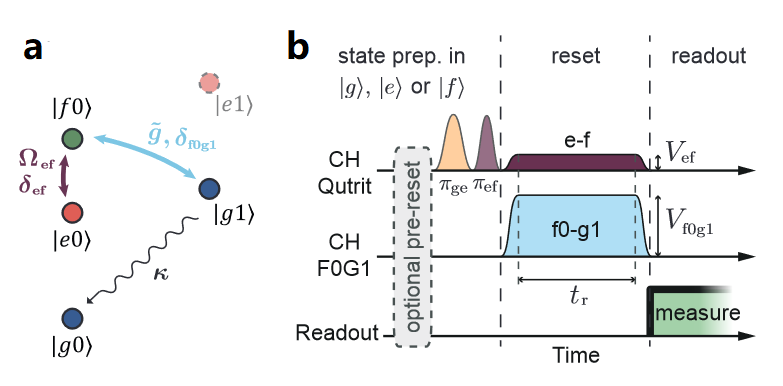
\includegraphics[width=0.7\textwidth]{reset2.png}
	\caption{施加GHz量级的微波实现比特状态重置示意图\cite{magnard2018fast}。a)利用GHz量级的微波实现比特状态重置的物理过程,通过微波将$\ket{10}$态,$\ket{20}$态和$\ket{01}$态进行耦合,实现能量的快速耗散。b)所施加的GHz量级微波波形示意图,实现比特和读取腔之间的能量转换。}
	\label{fig:reset2}
\end{figure}

\section{超导量子比特的状态操控}
完成初态制备后,我们要对初态进行状态操控,以此构成一个算法所需的幺正演化过程。利用单比特$R_X(\pi/2)$门和两比特CZ门就可以组成任意的幺正演化过程,下面主要介绍这两种门的具体实现方式。
\subsection{单比特$R_X(\pi/2)$门}
单比特$R_X(\pi/2)$门对应的矩阵形式为:
\begin{equation}
	 R_X(\pi/2)=\frac{1}{\sqrt{2}}\begin{pmatrix}
		1 & -i \\
		-i & 1
	\end{pmatrix}.
\end{equation}

电容耦合驱动控制的电路示意图如下图\ref{fig:drive}所示,据此可推导出系统的量子化哈密顿量为:
\begin{equation}
	H = \dfrac{\hat{Q}^{2}}{2C_{\Sigma}}-E_{J}\cos\left(\hat{\varphi}\right)+\dfrac{C_{d}}{C_{\Sigma}}V_{d}(t)\hat{Q},
\end{equation}
其中$ C_{d}$是驱动线与比特的耦合电容,$ C_{\Sigma}=C+C_{d}$是与比特耦合的所有电容的和。$V_{d}(t)$是驱动的交流电压,一般用余弦形式表示为$ V_{d}(t)=V_{0}\cos(\omega_{d}t+\phi)$,$ \omega_{d}$是驱动交流电压的频率,$ \phi$是驱动交流电压的相位。
\begin{figure}[h]
	\centering
	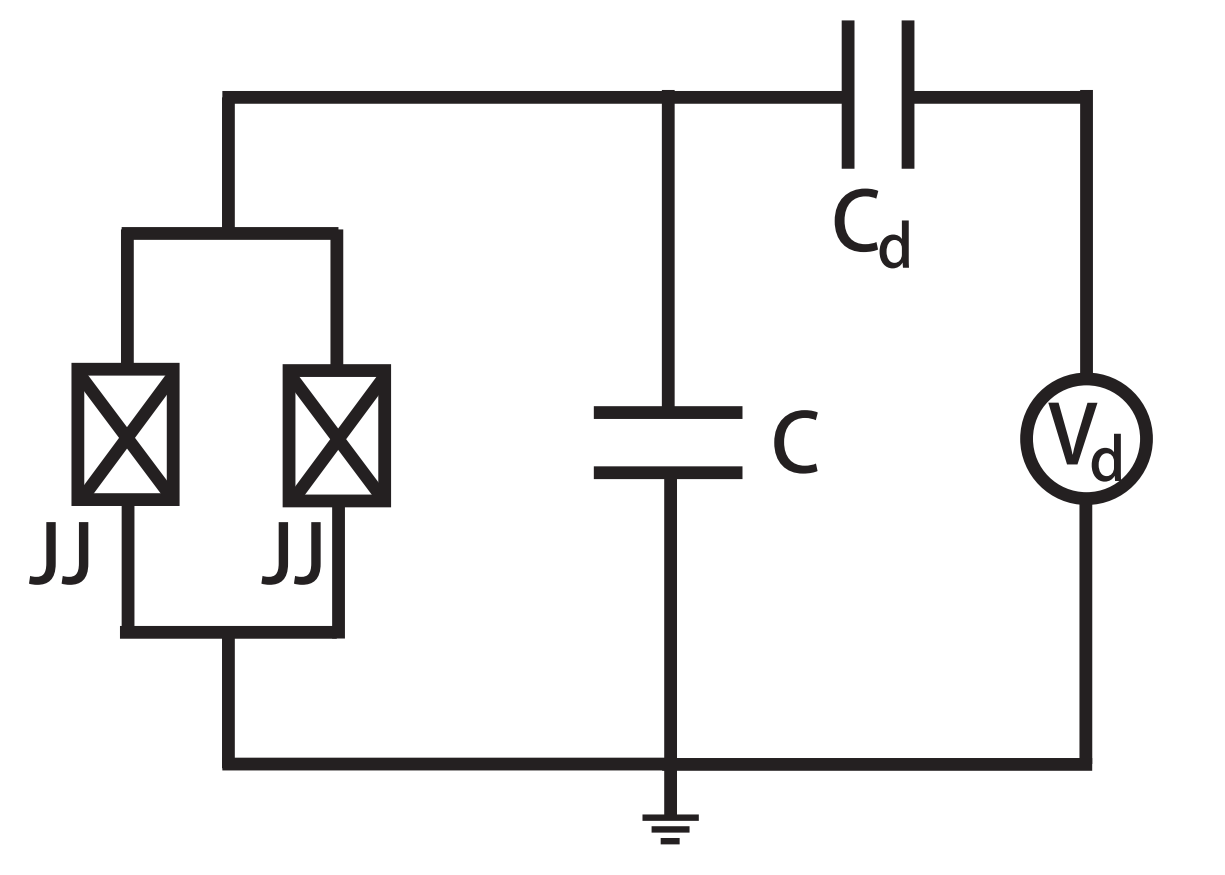
\includegraphics[width=0.7\textwidth]{Drive.png}
	\caption{电容耦合驱动控制的电路示意图。}
	\label{fig:drive}
\end{figure}
利用二次量子化方法,将整个系统转换到粒子数表象,并把哈密顿量截断到$ \ket{0}$和$ \ket{1}$展开的计算空间内,将产生、湮灭算符替换成对应的Pauli算符:$ a \rightarrow \sigma^{-}$,$ a^{\dagger} \rightarrow \sigma^{+}$,则系统哈密顿量的形式变为:
\begin{equation}
	H = -\dfrac{\hbar\omega}{2}\sigma^{z}+\dfrac{C_{d}V_{0}}{C_{\Sigma}}{e}(\dfrac{E_{J}}{2E_{C}})^{1/4}\cos(\omega_{d}t+\phi)\sigma^{y},
\end{equation}
其中$ \hbar\omega = \sqrt{8E_{C}E_{J}}-E_{C}$为量子比特的自身频率,$ E_{C} = \dfrac{{e}^{2}}{2C_{\Sigma}}$是量子比特的充电能。可以观察到耦合电容$ C_{d}$会影响量子比特的自身频率,但是实际量子比特设计中,$ C_{d}\ll C$,所以这种影响几乎可以忽略。

哈密顿量中的第一项是量子比特自身的静态哈密顿量,第二项就是电容耦合驱动的动态哈密顿量。在此动态哈密顿量的作用下,量子比特的状态绕着布洛赫球中的Y轴进行旋转,驱动强度$ g_{c}$定义为:$ \hbar g_{c} = \dfrac{C_{d}V_{0}}{C_{\Sigma}}{e}(\dfrac{E_{J}}{2E_{C}})^{1/4}$。经过替换后,系统哈密顿量可表示为:$ H = -\dfrac{\hbar\omega}{2}\sigma^{z}+\hbar g_{c}\cos(\omega_{d}t+\phi)\sigma^{y}$。

当驱动频率$ \omega_{d}$与比特频率$ \omega$相等时,经过旋转坐标系变换\cite{whaley1984rotating},系统的哈密顿量可以转化成:
\begin{equation}
	H_{r}/\hbar=-\dfrac{g}{2}(\cos\varphi\sigma^{x}-\sin\varphi\sigma^{y}),
\end{equation}
这是一个不含时哈密顿量,其演化矩阵$ U={e}^{-iH_{r}t/\hbar}={e}^{{i}\frac{gt}{2}(\cos\varphi\sigma^{x}-\sin\varphi\sigma^{y})}$,这个演化矩阵是一个标准的旋转算符。从布洛赫球表象上观察,其具体作用就是单比特状态绕着XY平面上的射线$ (\cos\varphi,-\sin\varphi,0)$为轴,旋转了角度$ gt$。此操作的旋转轴可以由驱动微波的相位$ \phi$调节,旋转角度可以由驱动微波的强度对时间的积分决定。当$ \varphi=0$时,实现了绕X轴正半轴旋转的操作;当$ \varphi=\pi/2$时,实现了绕Y轴正半轴旋转的操作。因此,当选择$ \varphi=0$,且驱动时间$t=\dfrac{\pi}{2g}$,即可构成一个$R_X(\pi/2)$门。
\subsection{两比特受控Z门}

双比特受控Z门(CZ门)的矩阵形式可以表示为:
\begin{equation}
CZ=\begin{pmatrix}
		1 & 0 & 0 & 0 \\
		0 & 1 & 0 & 0 \\
		0 & 0 & 1 & 0 \\
		0 & 0 & 0 & -1 
	\end{pmatrix}.
\end{equation}

根据CZ门的矩阵形式,需要在$\ket{11}$能级积累一个额外的$\pi$相位。我们通过两个能级间的相互排斥实现这个额外的相位积累,如下图\ref{fig:CZ}所示。
例如两个耦合比特的频率分别为$\rm 5.0$GHz和$\rm 4.875$GHz,非简谐性的大小为$-250$MHz,比特间耦合强度为$\rm 10$MHz。在进行做门操作时,需要对第二个比特施加类方波形式的快Z信号,以调节其比特频率,从而将系统的$\ket{11}$能级与$\ket{02}$能级相互靠近,二者之间的相互耦合使得$\ket{11}$能级与$\ket{02}$能级形成免交叉。通过这种方式,四个计算基矢只有$\ket{11}$被明显排斥,也因此其积累了额外的条件相位。当条件相位为$\rm \pi$时,就构成了一个受控相位Z门。

\begin{figure}[h]
	\centering
	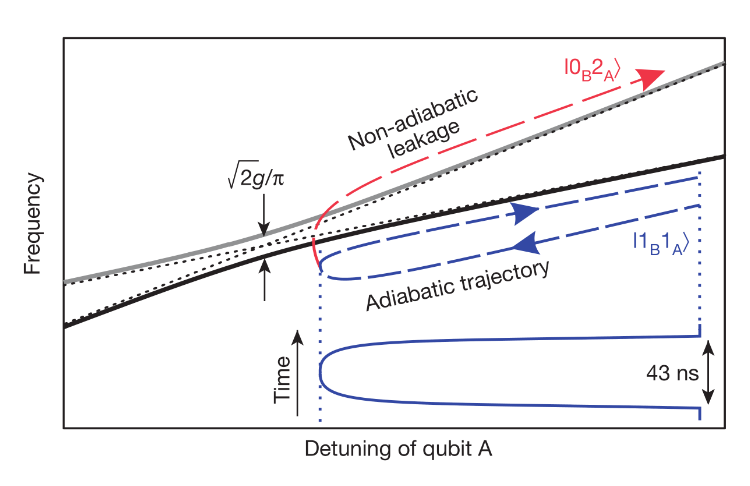
\includegraphics[width=0.7\textwidth]{CZ.png}
	\caption{通过$\ket{11}$能级与$\ket{02}$能级免交叉实现CZ量子门的示意图。}
	\label{fig:CZ}
\end{figure}




\section{超导量子比特的状态读取}
经过初态制备和量子门操作的量子计算过程后,还需要将量子计算的结果提取成经典信息,也就是对量子比特的状态进行测量。量子比特的测量方法有很多种,现在应用最广泛的方法是色散读取方法,这里主要介绍色散读取方法。
在色散读取中,量子比特与一个线性的谐振腔失谐耦合,二者的频率差远大于耦合强度。在这种条件下,量子比特的状态只会影响谐振腔的的频率,比特$ \ket{0}$态和$ \ket{1}$态分别对应谐振腔的两个频率。根据耦合体系的这种性质,当读取信号注入谐振腔,激发谐振腔能级的时候,不同的比特状态会使得读取信号获得不同的相位移动。读取信号离开谐振腔后,通过测量读取信号的相位,就可以获得量子比特的状态信息。
\subsection{二能级量子比特与读取腔的色散读取}
量子比特与谐振腔进行耦合,其电路模型如图\ref{fig:QR}所示。系统哈密顿量可以写为:
\begin{equation}
	H = -\dfrac{\hbar\omega_{q}}{2}\sigma^{z}+\hbar\omega_{r}a^{\dagger}a+hg(\sigma^{+}a+\sigma^{-}a^{\dagger}),
\end{equation}
其中$ \omega_{q}$和$\omega_{r}$分别是比特和谐振腔的频率,二者之间的频率差$ \Delta=\omega_{q}-\omega_{r}$。$ g$是比特和谐振腔之间的耦合强度。
在我们的设计中,耦合强度$g$远小于频率差$ \Delta$,经过坐标系旋转后可以得到耦合系统哈密顿量的近似表达式为:
\begin{equation}\label{approread}
	H'\approx H-\lambda[T,H]=-\dfrac{\hbar\omega_{q}}{2}\sigma^{z}+\hbar(\omega_{r}+\chi\sigma^{z})a^{\dagger}a,
\end{equation}
其中,$\chi=-\dfrac{g^{2}}{\Delta}$,即是所定义的色散位移。根据\ref{approread}式可以明显观察到,在$ g \ll \Delta$条件下,与比特耦合后的谐振腔频率$\omega_{r}^{'}=\omega_{r}+\chi\sigma^{z}$,这是一个与比特状态相关的物理量。当比特处于$\ket{0}$态时,谐振腔频率$\omega_{r}^{\ket{0}} = \omega_{r}+\chi$;当比特处于$\ket{1}$态时,谐振腔频率$\omega_{r}^{\ket{1}} =\omega_{r}-\chi$。不同比特状态下,读取谐振腔的频率不同,因此当读取信号经过读取谐振腔时,获得的相位移动也不相同。所以通过探测输出的读取信号的相位移动,可以测量量子比特状态。

\begin{figure}[h]
	\centering
	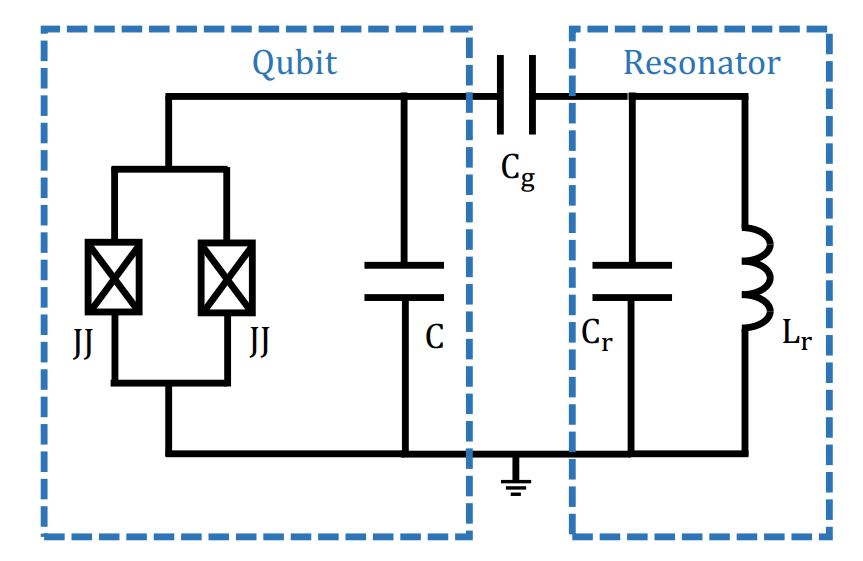
\includegraphics[width=0.7\textwidth]{QR.png}
	\caption{量子比特与读取腔电容耦合电路示意图。}
	\label{fig:QR}
\end{figure}

以上是二能级的量子比特与谐振腔耦合的结果,但是实际的传输子量子比特并不是一个单纯的二能级,而是具有非简谐性$ \eta$的多能级系统,所以第三能级同样也会影响读取腔的频率。如果考虑第三能级的影响,色散位移$ \chi$需要被修正为\cite{sank2014fast}:
\begin{equation}
	\chi = -\dfrac{g^{2}}{\Delta}\dfrac{1}{1+\Delta/\eta},
\end{equation}
量子比特在$\ket{0}$态和$\ket{1}$态时,谐振腔频率依然分别是$\omega_{r}+\chi$和$\omega_{r}-\chi$。
\subsection{读取信号的相位移动}
接下来介绍谐振腔色散位移对读取信号相位移动的具体影响。考虑到读取信号和谐振腔的相互作用只是经典力学框架下的相互作用,读取信号注入到谐振腔的物理过程可以由图\ref{fig:ReadoutS21}表示。
当读取信号通过传输线传输到谐振腔与传输线的耦合位置时,由于读取腔与传输线的耦合,耦合部分的阻抗不再等于传输线的特征阻抗$ Z_{0}$。阻抗不匹配使得读取信号在耦合位置产生透射和反射,透射的强度由散射参数$ S_{21}$表征,即输出信号与输入信号强度的比值$ S_{21} = \dfrac{V_{out}}{V_{in}}$,$S_{21}$是一个复数。读取谐振腔的频率会影响耦合位置的阻抗,进而影响读取信号的$S_{21}$。所以通过测量整个读取线路的散射参数$S_{21}$,可以表征出对应读取谐振腔的频率特性,进而测量量子比特的状态。
\begin{figure}[h]
	\centering
	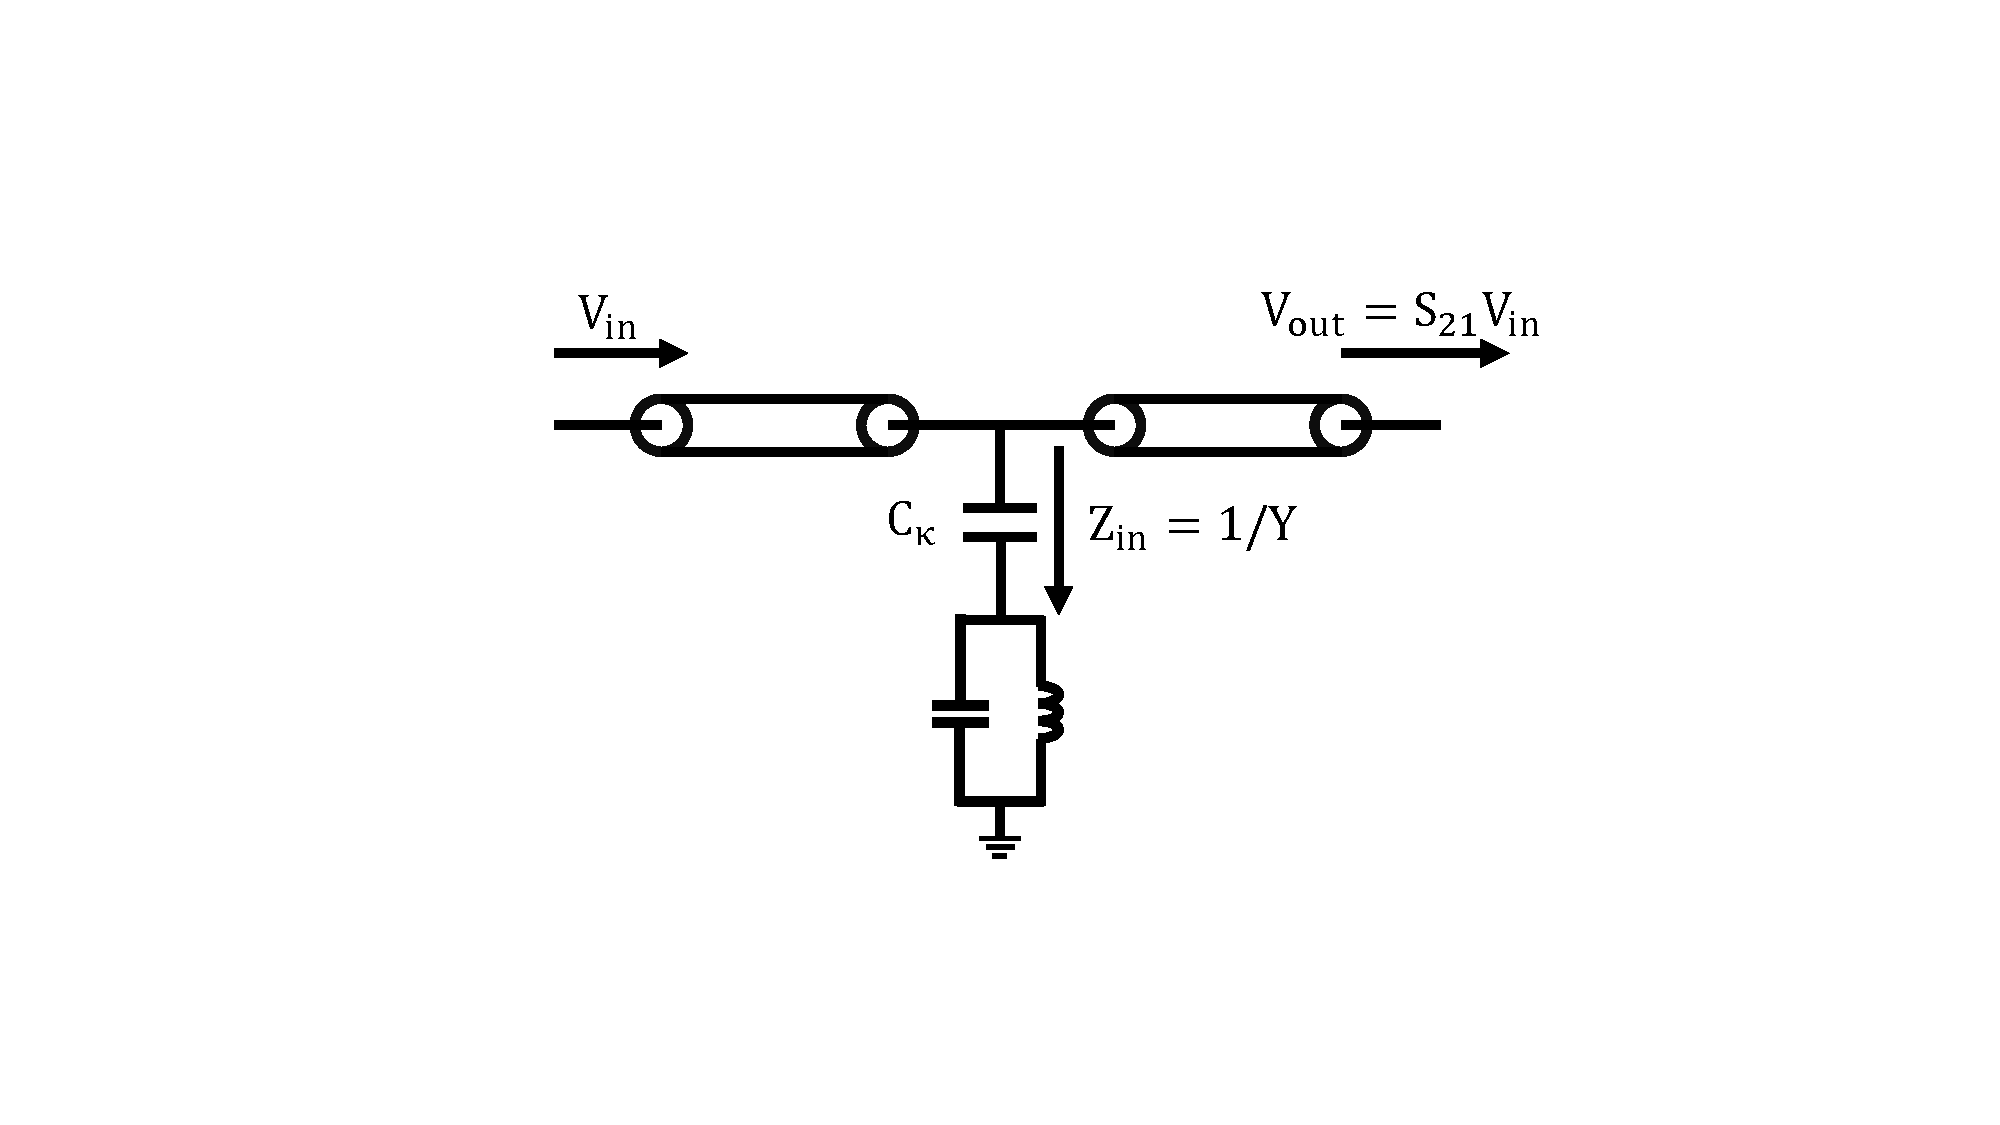
\includegraphics[width=0.7\textwidth]{ReadoutS21.pdf}
	\caption{被读取谐振腔分流的读取信号传输线路示意图。输入的读取信号电压幅度为$ V_{in}$,当读取信号传输到读取谐振腔所在的位置时,由于读取腔与传输线路的耦合,这一耦合部分的阻抗不再等于传输线特征阻抗$ Z_{0}$,因此阻抗不匹配使得读取信号产生透射和反射。透射的强度由$S_{21}$表征。读取谐振腔的频率影响阻抗$ Z_{in}$,进而影响读取信号的$ S_{21}$。通过测量$S_{21}$表征读取谐振腔的频率,进而表征比特状态。}
	\label{fig:ReadoutS21}
\end{figure}

根据微波的传输特性,读取微波信号在耦合部分的散射参数$S_{21}=\frac{2Z_{in}}{2Z_{in}+Z_{0}}$\cite{pozar2011microwave}。其中$ Z_{0}=50\  \Omega$为传输线的特征阻抗,$Z_{in}$是分流线路的阻抗,即谐振腔与耦合电容$ C_{\kappa}$构成系统的阻抗。据此公式,可以得到读取微波信号的散射参数$S_{21}$,及其实部、虚部分别为\cite{mazin2005microwave,megrant2012planar}:
\begin{align}\label{s21read}
	S_{21} &= \dfrac{S_{min}+2{i}Q_{l}\delta y}{1+2{i}Q_{l}\delta y},\\
	ReS_{21} &= \dfrac{S_{min}+(2{i}Q_{l}\delta y)^{2}}{1+(2{i}Q_{l}\delta y)^{2}},\\
	ImS_{21} &= \dfrac{2Q_{l}\delta y (1-S_{min})}{1+(2{i}Q_{l}\delta y)^{2}},
\end{align}
其中$ Q_{l}^{-1}=Q_{i}^{-1}+Q_{c}^{-1}$,$ Q_{i}$是谐振腔内在品质因数,表征谐振腔通过自身损耗源损耗的能量大小,$Q_{c}$是谐振腔耦合品质因数,表征谐振腔通过耦合的传输线泄露的能量大小,$S_{min}=Q_{c}/(Q_{c}+Q_{i})$,$ \delta y = (\omega-\omega_{r})/\omega_{r}$。
假设读取信号的频率为$\omega=(\omega_{r}^{\ket{0}}-\omega_{r}^{\ket{1}})/2$,将其带入方程\ref{s21read},可以观察到$ S_{21}$的实部是相同的,虚部互为相反数。从IQ复平面的角度分析,$\ket{0}$态和$\ket{1}$态的读取信号分别位于X轴上下两侧,关于X轴对称。通过在复平面对读取信号散射参量$ S_{21}$进行分析,可以明显区分$\ket{0}$态和$\ket{1}$态对应的读取信号,最终两个状态的读取信号分布如图\ref{fig:IQ}所示。


\begin{figure}[h]
	\centering
	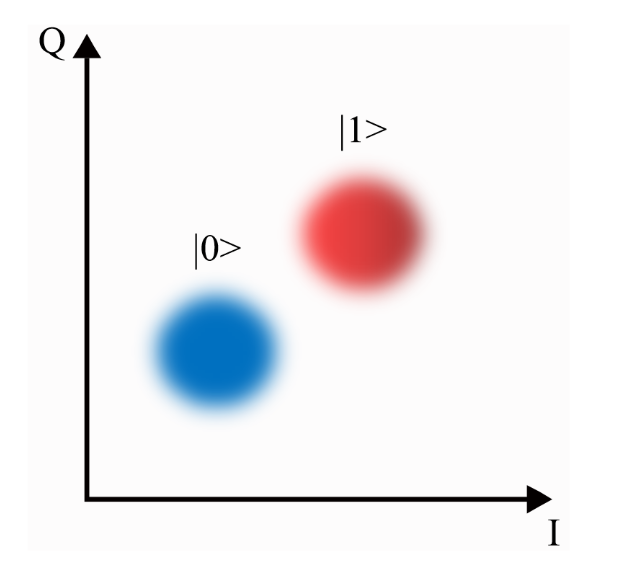
\includegraphics[width=0.7\textwidth]{IQ.png}
	\caption{$\ket{0}$态和$\ket{1}$态对应测量结果示意图。}
	\label{fig:IQ}
\end{figure}

\subsection{量子比特状态读取结果的校准}
在具体实验中,量子比特状态的读取分为单发测量和系综测量两种方式。单发测量是对量子比特状态进行单独地一次测量。根据测量结果在IQ复平面上的位置确定量子比特是处于$\ket{0}$态还是$\ket{1}$态;系综测量是针对物理观测量的测量,需要对量子比特状态进行多次测量。根据多次测量结果在IQ平面上的分布确定量子比特在$\ket{0}$态和$\ket{1}$态的概率$ P_{\ket{0}}$和$ P_{\ket{1}}$,进而得到物理观测量的平均值。

单发测量获得的是单独的一个结果,很难进行结果的矫正,但是系综测量获得的是多次测量的一个统计平均结果,可以通过统计学的一些方式进行测量结果的校准。具体过程主要分为两步:

第一步是对读取的误差进行标定:先将量子比特制备到$\ket{0}$态,然后直接对其进行状态读取,获得初态在$\ket{0}$态时,测量结果为$\ket{0}$态和$\ket{1}$态的概率分别为$ F_{00}$和$ F_{01}$;同样的,将量子比特初态制备到$\ket{1}$态,利用相同的方法可以标定出初态为$\ket{1}$态,测量结果为$\ket{0}$态和$\ket{1}$态的概率分别为$F_{10}$和$ F_{11}$。根据这四个标定参数,可以对原始读取结果进行校准;

第二步是对原始的读取结果进行校准:根据$F_{00}$、$F_{01}$、$F_{10}$和$F_{11}$四个标定参数,可以构建矩阵${F_{c}}$:
\begin{equation}
	{F_{c}} = \left(\begin{array}{cc}
		F_{00}&F_{01}\\
		F_{10}&F_{11}
	\end{array}\right)
\end{equation}
整个矩阵的作用效果是将理想的$\ket{0}$态和$\ket{1}$态概率转化为实验测得的$\ket{0}$态和$\ket{1}$态概率。例如初态为$\ket{0}$态,则理想的测量结果应为$ P_{\ket{0}}=1$、$ P_{\ket{1}}=0$,但实际结果为$F_{00}$和$F_{01}$,相当于${P_{exp}}={F_{c}}{P_{ideal}}$,其中${P_{ideal}}$和${P_{exp}}$是由$ P_{\ket{0}}$和$P_{\ket{1}}$组成的矢量。
\begin{equation}
	{P_{ideal}} = \left(\begin{array}{c}
		P_{\ket{0}}^{ideal}\\
		P_{\ket{1}}^{ideal}
	\end{array}\right),
	{P_{exp}} = \left(\begin{array}{c}
		P_{\ket{0}}^{exp}\\
		P_{\ket{1}}^{exp}
	\end{array}\right)
\end{equation}
因此,当进行系统测量时,如果概率测量结果为${P_{exp}}$,可以通过${P_{ideal}}={F_{c}^{-1}}{P_{exp}}$,得到理想的概率测量结果${P_{ideal}}$。这就是量子比特状态读取结果的校准方法。

\section{总结}
上一章介绍了超导量子计算系统的基本构成和基本原理。本章在此基础之上,介绍如何对超导量子比特的状态进行操控和测量,例如量子比特的初态制备,单比特和双比特门操作以及量子状态的色散测量,以此构成一个完整的量子计算过程。